\subsection{Medical Background}
\label{subsec:med_background}

\subsubsection{Blood Pressure}
\label{subsubsec:bp}

% general BP
Blood pressure (BP) is a physiological measure of the force exerted by circulating blood against the walls of the arteries~\cite{WhatBloodPressure2019}.
It is highly dependent on blood flow, which refers to the movement of blood through a vessel, tissue, or organ.
Blood circulation begins with the contraction of the heart's ventricles.
This action generates a type of hydrostatic pressure, which is the force exerted by a fluid due to gravitational pull, typically against the walls of the container that confines it.

BP is a type of hydrostatic pressure, representing the force exerted by blood on the walls of blood vessels or the heart's chambers.
While it can be assessed in various body regions, the term \enquote{blood pressure} without specific qualifiers commonly refers to systemic arterial BP\@.
This denotes the pressure of blood within the arteries of the systemic circulation.
In clinical settings, this pressure is measured in millimeters of mercury (mmHg) and is typically acquired using the brachial artery in the arm~\cite{betts20BloodFlow2022}.

% measuring significance
Measuring BP is crucial for assessing cardiovascular health and identifying potential risks.
It allows for the early detection of conditions like hypertension and hypotension, enabling timely interventions to prevent serious cardiovascular events~\cite{naylorArterialCathetersEarly2020}.
BP serves as a key indicator of the risk for heart attacks, strokes, and heart failure, guiding preventive measures and treatment strategies~\cite{ettehadBloodPressureLowering2016}.

\vspace{0.2cm}
\textit{Various Types of Measurement}
\vspace{0.2cm}

% cuff BP measuring TODO: add images of sphygmanometer, ABP cathether etc.
One of the most common BP measurement methods is one using a sphygmomanometer, also known as non-invasive blood pressure (NIBP), is typically recorded as numeric values at specific time intervals.
The process involves inflating the cuff to temporarily stop blood flow and then gradually releasing the pressure to detect the sounds associated with the flow of blood through the brachial artery.
The two primary values obtained are systolic pressure (maximum pressure during heartbeats) and diastolic pressure (minimum pressure between heartbeats).
During the process of cuff inflation and deflation, each heartbeat generates characteristic sounds (Korotkoff sounds) that are detected by a stethoscope placed over the brachial artery.
Systolic pressure is recorded when the first tapping sounds are heard, and diastolic pressure is recorded when the sounds disappear or change character.
This beat-to-beat approach provides information about individual fluctuations in blood pressure~\cite{betts20BloodFlow2022}.

While measuring blood pressure with a cuff using a sphygmomanometer is a common and convenient method, it has its limitations as it cannot be done continuously.
This intermittent approach provides valuable insights into systolic and diastolic pressures at specific time intervals, but it may not capture the nuanced changes that occur between measurements.
To address the need for continuous monitoring, other methods, such as arterial catheterization, are employed.

% arterial BP
Arterial catheterization is commonly employed in critical patient care, serving dual purposes: continuous blood pressure monitoring and obtaining frequent blood gas measurements.
Typically conducted at bedside, the procedure utilizes percutaneous methods like the Seldinger technique to cannulate arteries~\cite{clarkArterialCatheterization1992}.
The resulting arterial blood pressure (ABP) is a dynamic parameter that can change with each heartbeat, and it is typically represented as a waveform rather than a single numeric value.
The ABP waveform consists of two main components: systolic pressure and diastolic pressure.
Such continuous monitoring of ABP is usually done in clinical settings, using an arterial line connected to a pressure transducer.
The resulting waveform is displayed on a monitor in real-time.
However, for ease of interpretation and documentation, numeric values are commonly extracted from the waveform at specific time intervals~\cite{hillImputationContinuousArterial2021}.

In situations where high temporal resolution is crucial, ABP can be recorded beat-to-beat, providing a value for each heartbeat.
This is particularly important in situations where rapid changes in blood pressure need to be closely monitored, such as during certain medical procedures or in critically ill patients~\cite{lehmanMethodsBloodPressure2013}.

For routine monitoring and documentation, numeric values are often averaged over a specific time interval, such as every 1, 5, or 15 minutes.
This averaged value may be reported as the mean arterial pressure (MAP), which is a weighted average of the systolic and diastolic pressures over a cardiac cycle~\cite{demersPhysiologyMeanArterial2024}
Some monitoring systems may also provide systolic and diastolic blood pressure readings at regular intervals.

Alternative approaches for measuring BP have emerged over the past years.
Volume clamping~\cite{kimBallistocardiogramBasedApproachCuffless2018} and tonometry~\cite{imholzFifteenYearsExperience1998} are some of the other methods.
These non-invasive techniques offer continuous monitoring of blood pressure values.
Volume clamping, which involves the use of a small finger cuff and a PPG sensor, is one method for continuous blood pressure measurement.
Tonometry, on the other hand, is a cuffless approach that utilizes a manometer-tipped probe pressed directly on an artery.
The volume clamping approach allows for instantaneous and prolonged blood pressure measurement.
However, it is associated with high costs and still necessitates the use of a cuff, which can be inconvenient and uncomfortable.
Conversely, the tonometry method is sensitive to movement of the arm and probe, making it challenging to maintain accuracy in practical applications.
Additionally, constant calibration with a cuff blood pressure device is required~\cite{peterReviewMethodsNoninvasive2014}.

\vspace{0.2cm}

In conclusion, blood pressure serves as a critical physiological measure, representing the force exerted by blood on the walls of blood vessels.
The conventional method of measuring blood pressure with a cuff and sphygmomanometer provides valuable insights into systolic and diastolic pressures but is limited by its intermittent nature.
To address the need for continuous monitoring, arterial catheterization is commonly employed in critical care, offering real-time data through a dynamic waveform.
Alternative non-invasive approaches like volume clamping and tonometry aim to provide continuous blood pressure monitoring, but they come with their own challenges and considerations.
As technology advances, these methods contribute to a comprehensive understanding of blood pressure dynamics, facilitating improved patient care and risk assessment.

\subsubsection{Photoplethysmography}
\label{subsubsec:ppg}

% meaning and basic information
Photoplethysmography (PPG) is an optical measurement technique designed to identify changes in blood volume within the microvascular bed of tissue~\cite{challonerPhotoelectricPlethysmographMeasurement1974}.
Its clinical application is extensive, as the technology is integrated into commercially available medical devices, including pulse oximeters, vascular diagnostics, and digital beat-to-beat blood pressure measurement systems.
The fundamental structure of PPG technology is straightforward, requiring only a few opto-electronic components: a light source for tissue illumination, usually a light-emitting diode (LED) and a photodiode (PD) to gauge slight variations in light intensity correlated with changes in perfusion in the catchment volume.

% history and origins
\vspace{0.2cm}
\textit{History}
\vspace{0.2cm}

One of the first mentioned instances on the use of PPG were recorded in 1936 by Molitor and Kniazuk~\cite{molitorNewBloodlessMethod1936}.
They outlined comparable devices employed for tracking alterations in blood volume in the rabbit ear under conditions of venous occlusion and the administration of vasoactive drugs.
A pioneer who helped establish the PPG technique was Alrick Hertzman~\cite{hertzmanPhotoelectricPlethysmographyFingers1937}.
In his 1937 paper, Hertzman coined the term \enquote{Photoelectric Plethysmograph} etymologically meaning:
photo - \enquote{light}, plethora - \enquote{exess of body fluid, blood}, graph - \enquote{something written}.
He detailed the application of a reflection mode system to assess alterations in blood volume within the fingers, particularly during the Valsalva maneuver~\cite{srivastavValsalvaManeuver2024}, exercise, and exposure to cold.
This contribution not only demonstrated the versatility of the technique but also underscored its potential clinical relevance.

Hertzman and Spealman~\cite{hertzmanPhotoelectricPlethysmographyFingers1937} outlined two crucial features of the PPG pulse waveform.
They categorized the pulse appearance into two phases: the anacrotic phase representing the ascending edge of the pulse, and the catacrotic phase representing the descending edge of the pulse.
The initial phase primarily corresponds to systole, while the subsequent phase relates to diastole and wave reflections from the periphery.
In individuals with healthy compliant arteries, a dicrotic notch is commonly observed during the catacrotic phase.

In the late 1970s, there arose a renewed interest in the PPG technology, driven by the demand for compact, dependable, cost-effective, and user-friendly noninvasive cardiovascular assessment techniques~\cite{yoshiyaSpectrophotometricMonitoringArterial1980}.
The progress in opto-electronics and clinical instrumentation has played a significant role in advancing PPG technology.
Semiconductor advancements, particularly in LEDs, photodiodes, and phototransistors, have brought about substantial improvements in the size, sensitivity, reliability, and reproducibility of PPG probe design.
A significant leap in the clinical application of PPG-based technology occurred with the introduction of the pulse oximeter~\cite{aoyagiPulseOximetryIts2002}.
This device revolutionized non-invasive monitoring of patients' arterial oxygen saturation, marking a major advancement in the field.

Other emerging technologies encompass PPG imaging technology, telemedicine, and remote monitoring.
In 2005, Wieringa et al.\ detailed a contactless multiple-wavelength PPG imaging system designed primarily for remotely imaging the distribution of arterial oxygen saturation (SpO2) within tissue~\cite{wieringaContactlessMultipleWavelength2005b}.
The system captures movies of two-dimensional matrix spatially resolved PPG signals at different wavelengths during respiratory changes.
PPG was found to have substantial potential in telemedicine, particularly for remote/home health monitoring of patients.
Miniaturization, user-friendliness, and robustness stand as pivotal design criteria for such systems.
This is exemplified by finger ring-based PPG sensors for monitoring beat-to-beat pulsations (\cite{rheeArtifactresistantPowerefficientDesign2001}, ~\cite{zhengRingtypeDeviceNoninvasive2003}).

Most PPG devices these days either use the transmissive or reflective operating modes (illustrated in Figure~\ref{fig:reflection}).
Currently, the prevalent method is the transmissive mode, chosen for its notable accuracy and stability~\cite{leeReflectancePulseOximetry2016}.
However, there is a growing interest in reflective-mode PPG due to its elimination of the need for a thin measurement site.
This method proves versatile, applicable to various sites such as the feet, forehead, chest, and wrists.
Especially when the wrist serves as the designated measurement site, PPG sensors can be conveniently employed in the form of a band or watch.

\begin{figure}[h]
    \centering
    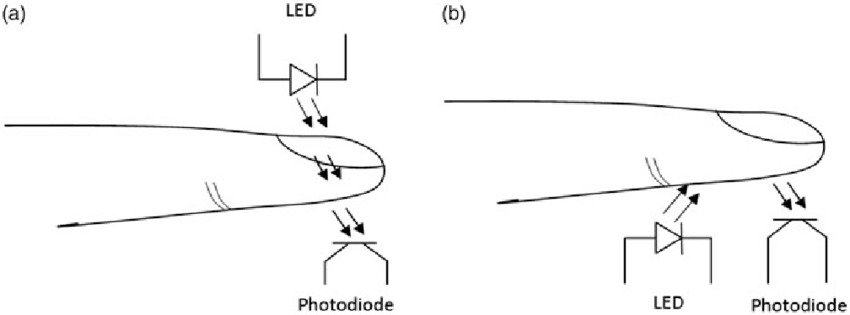
\includegraphics[scale=0.4]{images/ppg/reflection}
    \caption{PPG Transmission (a) and Reflection (b) operating modes \cite{mohanSpotMeasurementHeart2016}}
    \label{fig:reflection}
\end{figure}

% how does it work
\vspace{0.2cm}
\textit{Working Principle}
\vspace{0.2cm}

The PPG signal consists of pulsatile (AC) and superimposed (DC) components (see Figure~\ref{fig:acdc}).
The AC component originates from variations in blood volume associated with heartbeats,
while the DC component is influenced by factors such as respiration, sympathetic nervous system activity, and temperature regulation~\cite{allenPhotoplethysmographyItsApplication2007a}.
The AC component specifically illustrates changes in blood volume during phasic cardiac activity, representing both the systolic and diastolic phases.
The systolic phase, also known as the \enquote{rise time}, initiates with a valley and concludes at the pulse wave systolic peak.
The pulse wave concludes with another valley at the end of the diastolic phase~\cite{weisslerSystolicTimeIntervals1968}.
In most PPG waveform analyses including this one, the AC component in the form of a waveform signal is used.

\begin{figure}[h]
    \centering
    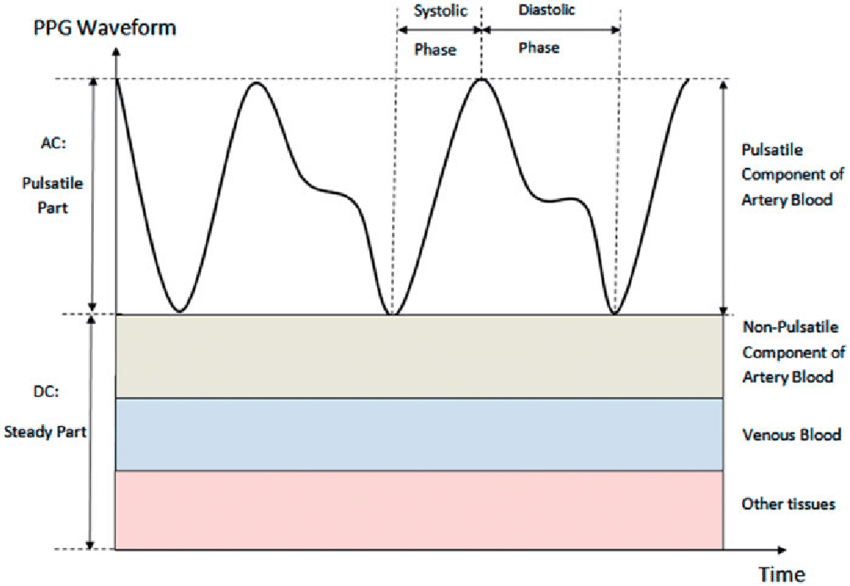
\includegraphics[scale=0.5]{images/ppg/ac+dc}
    \caption{AC and DC components of the PPG signal \cite{mohanSpotMeasurementHeart2016}}
    \label{fig:acdc}
\end{figure}

% main and potential use cases
\vspace{0.2cm}
\textit{Use Cases}
\vspace{0.2cm}

PPG finds diverse applications in clinical settings, covering physiological monitoring (such as blood oxygen saturation and heart rate), vascular assessment (including arterial disease, aging and tissue viability), and autonomic function evaluations (such as thermoregulation, heart rate and other assessments of cardiovascular variability)~\cite{allenPhotoplethysmographyItsApplication2007a}.
Furthermore, the popularity of PPG technology as an alternative for monitoring heart rate has risen recently, primarily attributed to its ease of use, user-friendly wearing comfort, and cost-effectiveness~\cite{sviridovaHumanPhotoplethysmogramNew2015}.
Nowadays, almost every wearable devices uses the PPG technology to track the user's heart rate and other extractable vital parameters~\cite{castanedaReviewWearablePhotoplethysmography2018}.
PPG sensors in mobile and wearable devices typically feature red, green, or both light-emitting diodes.
Most devices incorporate a green-light PPG sensor for continuous heart rate monitoring during daily activities.
Some devices also include red-light PPG sensors, which are effective for measuring heart rate when a person is stationary, providing insights into hydration, muscle saturation, and total hemoglobin.
While red-light PPG can penetrate tissue layers more deeply using near-infrared spectroscopy, it is susceptible to disturbance from ambient light.
In contrast, green light, being less absorbed by the skin, minimizes the impact of ambient light noise on the heart rate signal.
As a result, wearable devices commonly utilize green light rather than red-light PPG~\cite{ponnadaTechnologicalConsiderationsSensorassisted2019}.
Different types of devices implement the PPG technology.
It can be found in pulse oximeters, smartphones, smartwatches and other wearable devices (examples in Figure~\ref{fig:ppg-devices}).

\begin{figure}[h]
    \centering
    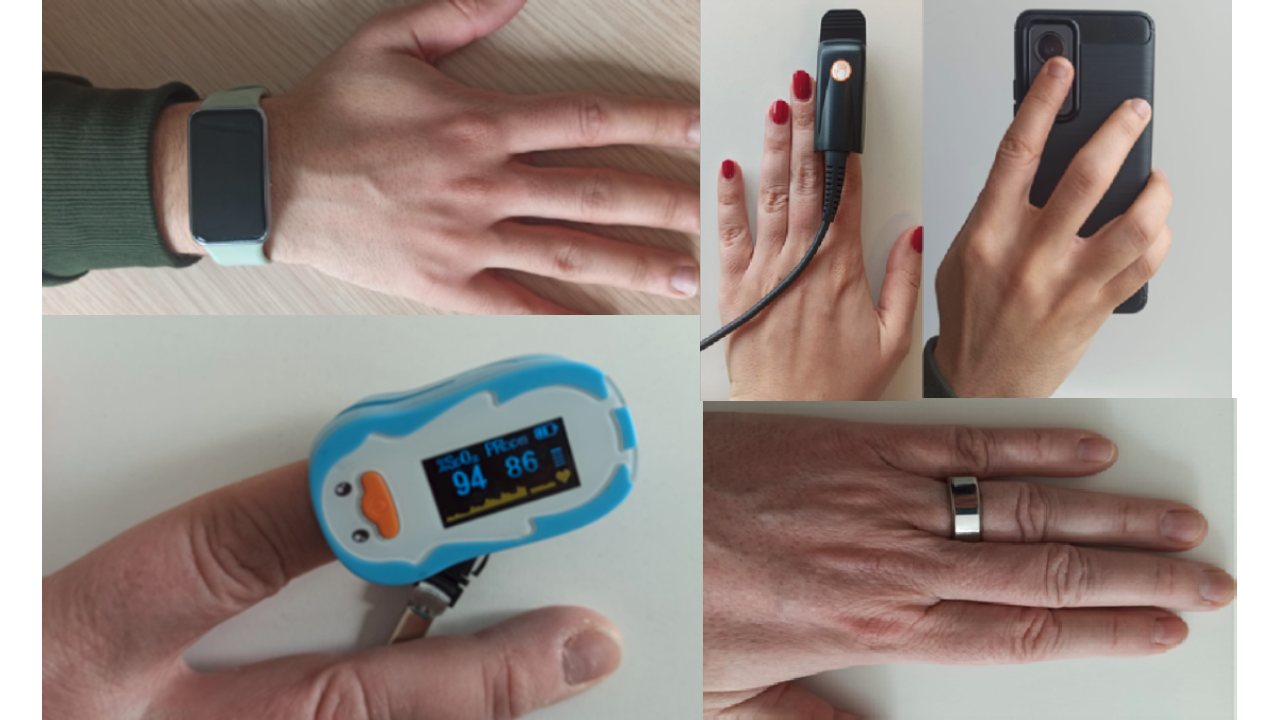
\includegraphics[scale=0.35]{images/ppg/ppg-devices}
    \caption{AC and DC components of the PPG signal \cite{zanelliPotentialAIBased2023}}
    \label{fig:ppg-devices}
\end{figure}

% Conclusion parahraph
\vspace{0.2cm}

In conclusion, the PPG is an optical sensor, consisting of an LED paired with a PD, hence it is simple, inexpensive and can be easily build into a wearable device.
The PPG waveform can be obtained using two modes, reflectance and transmission.
This waveform corresponds to the blood volume in blood vessels.
Traditionally employed in healthcare for heart rate and blood oxygen saturation measurements, particularly with pulse oximeters, the PPG plays a pivotal role~\cite{allenPhotoplethysmographyItsApplication2007a}.

% outlook to SP and ML
Additionally, peripheral volumetric changes exhibit correlation with BP~\cite{langewoutersPressurediameterRelationshipsSegments1986}.
Utilizing characteristic PPG features, machine learning functions can estimate Systolic BP (SBP) and Diastolic BP (DBP).
However, establishing a simple, clear, and continuous relationship between these features and BP remains elusive.
This method heavily relies on signal pre-processing, feature extraction, and the application of machine learning algorithms for BP estimation based on these features.

\subsubsection{MIMIC-III}
\label{subsubsec:mimic3}

origin of MIMIC\@.
When was it created?
How is it structured?

\subsubsection{MIMIC-IV}
\label{subsubsec:mimic4}

Multiparameter Intelligent Monitoring in Intensive Care IV (MIMIC-IV)~\cite{johnsonMIMICIVFreelyAccessible2023}.

\begin{enumerate}
    \item How is the database structured?
    \item Which patients and how many of them have both PPG and BP data?
    \item Arterial Blood Pressue (ABP)
\end{enumerate}

How does it differ from MIMIC3?

\subsection{Computing Background}
\label{subsec:computing_background}

\subsubsection{Signal Processing}
\label{subsubsec:signal_processing}

\begin{enumerate}
    \item What are the methods of signal processing for reading PPG?

    Approaches for processing the given PPG data in correlation to BP:\newline

    \textbf{Time (PTT) based on PPG \& ECG - Inverse correlation between BP and PTT.} PTT is the time delay for the pressure wave to travel between to sites on the body. It can be calculated as the time difference between proximal and distal waveforms indicative of the arterial pulse.

    \textbf{Pulse Arrival Time (PAT) = PTT + pre-ejection period.} It is defined as the time that takes the pulse wave to travel from the heart to a peripheral site e.g. finger, toe, etc. It can simply be estimated as the time delay between the R peak of the ECG waveform and a point on the rising edge of a distal PPG waveform.

    These methods require simultaneous measurement at two different sites on the body, hence two measurement sensors (ECG and PPG) are needed for recording the signals in order to estimate these parameters.

    \item What are the different types of filters for processing the PPG signal?

    Signal filtering types include: Chebyshev filter, Butterworth filter~\cite{liangOptimalFilterShort2018}.

    Savitzky-Golay (SG) filter~\cite{savitzkySmoothingDifferentiationData1964}

    Second derivative \& Age analysis~\cite{takazawaAssessmentVasoactiveAgents1998a}

    Hemodynamics and vascular age~\cite{charltonAssessingHemodynamicsPhotoplethysmogram2022}

\end{enumerate}

\subsubsection{Machine Learning}
\label{subsubsec:machine_learning}

\begin{enumerate}
    \item What are the methods of machine learning for estimating BP from PPG?
\end{enumerate}

Approaches for estimating BP from PPG: \newline

BP estimation using ML techniques is data driven, unlike the traditional PTT/PAT only models.
Several studies attempted to fit regression models, such as \textbf{multilinear regression, support vector machine and random forest}, for estimating BP using PTT/PAT based approach with some degree of success, but the results did not always satisfy the international standards.\newline

Teng and Zhang~\cite{tengContinuousNoninvasiveEstimation2003} tried to fit a \textbf{linear regression} model to study the relationship between four PPG features and BP. It was reported that the diastolic time has higher correlation with SBP and DBP than the other features.

Suzuki and Oguri~\cite{suzukiCufflessBloodPressure2009} used \textbf{AdaBoost} classifier for the estimation of BP. In this technique, SBP values were classified according to a threshold and afterwards the nonlinear machine learning model was employed for estimating SBP\@.

Ruiz-Rodriguez et al.~\cite{ruiz-rodriguezInnovativeContinuousNoninvasive2013} employed a probabilistic generative model, \textbf{Deep Belief Network Restricted Boltzmann Machine}, for predicting SBP, DBP and mean arterial pressure simultaneously.
The results of this study were highly variable, and therefore was not reliable.

Kurylyak et al. \cite{kurylyakNeuralNetworkbasedMethod2013} extracted 21 characteristic features from the PPG waveform.
These features were used for estimating SBP and DBP using a \textbf{feed forward neural network}.
The results were promising towards an accurate cuffless BP monitoring.

Xing and Sun~\cite{xingOpticalBloodPressure2016} applied \textbf{Fast Fourier Transformation} for selecting frequency domain features from the PPG waveform followed by a \textbf{feed forward neural} network for BP estimation.
However, the authors suggested that these features are not sufficient for effective BP estimation.

Liu et al. \cite{liuIntegratedNavigationTethered2017}, added 14 features extracted from the PPG’s second derivative, in addition to the 21 features used in Kurylyak et al.
A \textbf{support vector machine (SVM)} was then applied for estimating SBP and DBP\@.
The authors reported that these 14 features further improved the estimation.\newline

The relationship between BP and PPG features is not always linear.
Therefore, linear models are inappropriate and often fail to model the relationship between BP and PPG when tested on a large dataset collected from a diverse population.
Other classical machine learning models, such as \textbf{SVM}, and \textbf{random forest}, provide better precision.
Estimation using these models requires establishing one model per objective, hence, SBP and DBP are estimated separately.
However, DBP strongly correlates with SBP and improve its estimation [49], thus should be modelled simultaneously using one model architecture.
This can be achieved using neural networks. \textbf{Neural network} models can leverage large amount of data faster and more accurately compared to classical machine learning models.

El-Hajj and Kyriacou proposed using \textbf{Bidirectional Long Short-term memory (Bi-LSTM) and Bidirectional Gated Recurrent Units (Bi-GRU) with attention mechanisms}~\cite{el-hajjDeepLearningModels2021}.

In Su et al.~\cite{suLongtermBloodPressure2018}, a four layers \textbf{LSTM} with bidirectional structure and residual connections has been employed for BP estimation using the PTT approach.
The reported results outperform other PTT based BP regression models.

A study by Joung et al.~\cite{joungContinuousCufflessBlood2023} was conducted to evaluate a learning-based cuffless BP estimation system with calibration in challenging circumstances.
A one dimensional CNN-based network was designed, that could efficiently extract BP from PPG signals using a comparative paired 1D-CNN structure with calibration.

To precisely design a learning-based BP estimation model such that its estimation accuracy obtained during the test is sustained after being built upon a practical cuffless BP monitoring system, the following delicate yet realistic experimental principles are applicable:
i) the number of subjects should be sufficiently large,
ii) subject independent training and test datasets are required, and
iii) the intrasubject BP variation should be carefully scrutinized in the model design~\cite{joungContinuousCufflessBlood2023}.